\section{Synthesis of the equivalent transmission for full pupil illumination}
\label{sec:pupil_stitching}

The reflectivity of the telescope and the transmission of the filters
both exhibit a distinct radial dependency. Although the filter
transmission dependence is expected due to its interferometric nature,
the origin of the telescope reflectivity dependence remains
unclear. Despite this, we can construct an empirical model that
assumes smooth transitions between measurements and calculate the
theoretical "full pupil" transmission by averaging the model over the
illuminated portion of the primary mirror. These two steps are
necessary to achieve sub-percent color accuracy and sub-nanometer
precision in central wavelengths.

Finally, we estimate statistical and systematic errors on the final
transmission curves, propagating them through the analysis process. A
better understanding of these errors in interpreting broadband
photometry can be achieved by integrating them as uncertainties on
filter normalization and central wavelength, which can be easily
translated into errors in colors and color-terms.


\subsection{Radial model of the instrument transmission}
\label{sec:model}

The open transmission of the telescope is modeled as a smooth 2D
function of wavelength and incidence angle. The function is defined on
a basis of cubic B-splines, with \num{35} regularly spaced wavelength
nodes covering the range from \SIrange{350}{1100}{nm}, and two nodes
in angles corresponding to the inner and outer edges of the
occultation-free primary mirror, ranging from \SIrange{1.97}{7.24}
{\degree}. These angles represent radii of \SIrange{55}{203}{mm} for a
primary mirror with a focal length of \SI{1600}{mm}.

For data acquired using a filter, we multiply the open transmission
model by a model of the interference filter transmission, defined as
follows:
\begin{equation}
  \label{eq:filtertransmission}
T(\lambda, \theta) = \mathcal T\left(\frac{\lambda}{\sqrt{1 -
    (\sin(\theta) / n_\text{eff})^2}}\right)\,.
\end{equation}
Here, $n_\text{eff}$ is an effective index for the inserted filter,
and T is a piece-wise linear function of wavelength. The piece-wise
linear function is initially created with \num{150} regularly spaced
nodes between \SIrange{350}{1100}{nm}, providing a general resolution
of \SI{5}{nm}. In cases where more precision is needed, we further
refine the grid by equally splitting intervals where the local mean
chi-square exceeds the global mean chi-square by more than three
standard deviations. This process is repeated four times to ensure
that filter fronts are typically modeled with up to approximately
\SI{0.3}{nm} resolution.


Lastly, the photometry for the grating zeroth and first orders is
adjusted using a cubic B-spline model with \num{105} nodes in
wavelength.

The composite model is fit to dataset No.~2, which includes data
from four different radii and successive observations without filters
or with all seven filters and the grating. The baseline model has
\num{1979} free parameters: \num{148} for the open transmission,
approximately $6\times165$ for each of the $ugrizy$ filters, and
\num{420} for each of the grating orders. Unfortunately, the blue edge
of the $u$-band filters cannot be accurately determined by this
data. Fit results are displayed in
Fig.~\ref{fig:lambdathetafitresults}.

\begin{figure*}
  \centering
  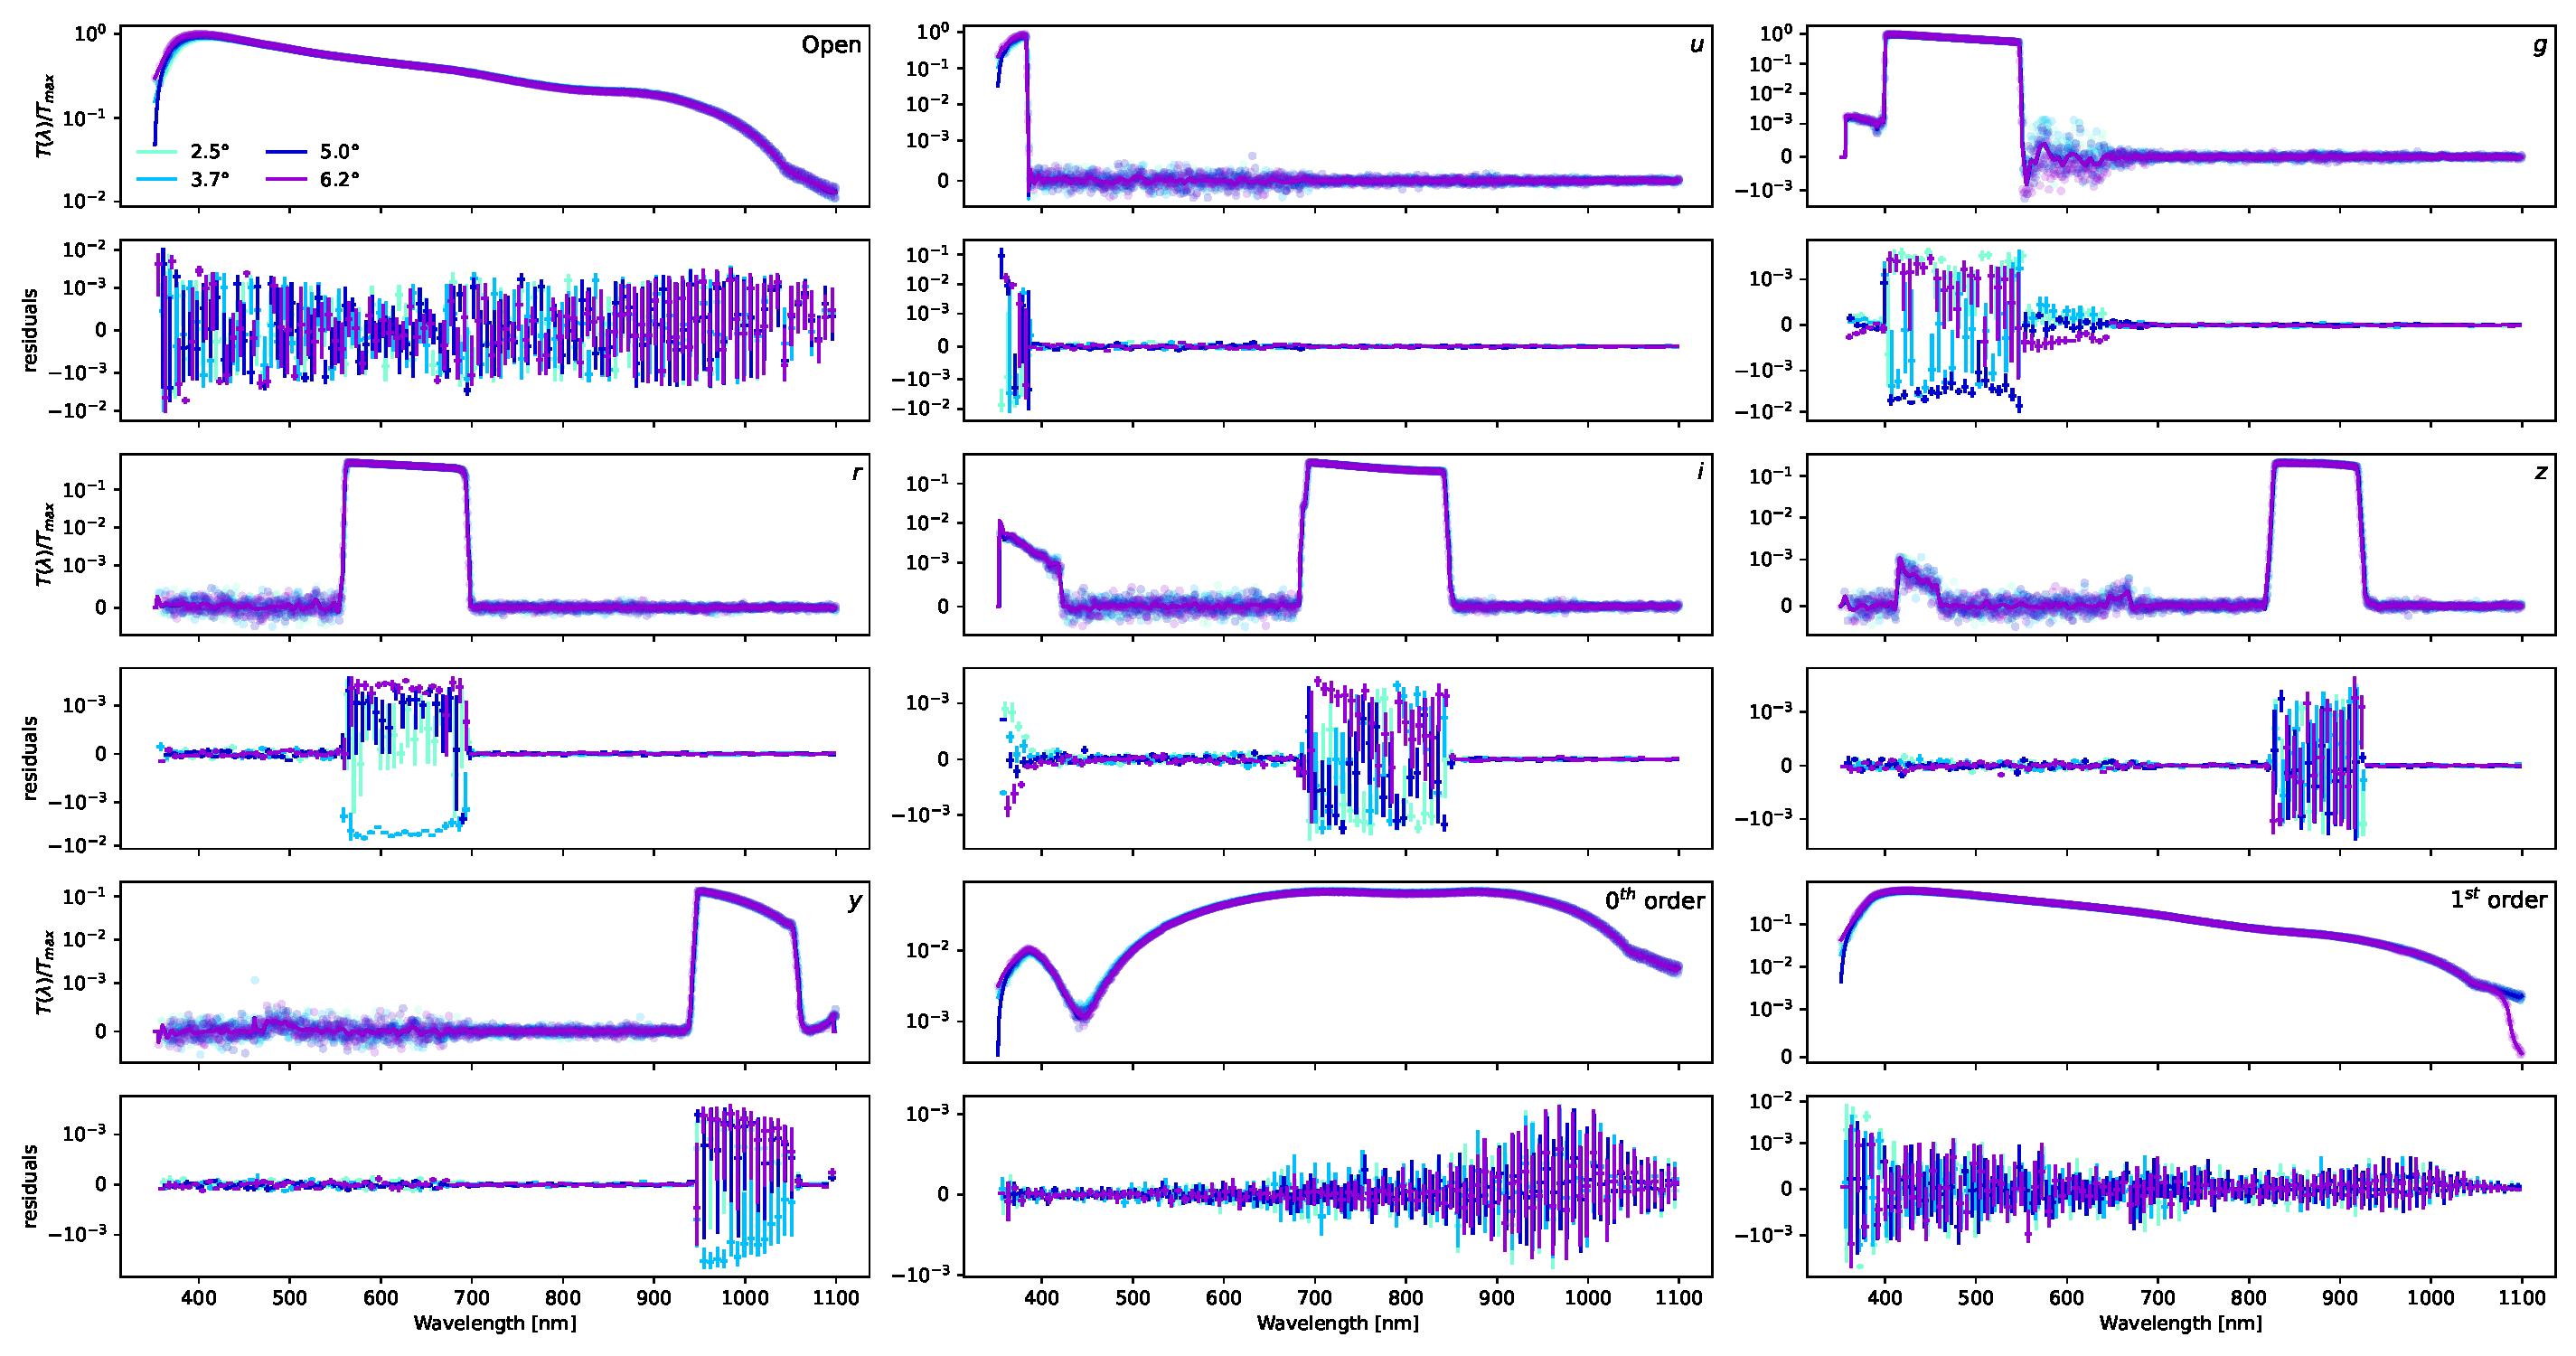
\includegraphics[width=1\linewidth]{./fig/lambdathetafitresults.pdf}
  \caption{Model of the wavelength and radial dependency of the
    StarDICE response to CBP illumination $R(\lambda)$ (see
    Eq.~\ref{eq:rtot}). Each panel display the raw measurements at the
    4 sampled position for each of the filter configurations: no
    filters (Open), with one of the 6 photometric filters ($ugrizy$)
    or with the grating looking either at the zeroth order or the
    first order spots. The panel immediately below each panel display
    the residuals to the model. For easy comparison, all panels are
    normalized to the peak of the response, which occurs in the open
    configuration at $\lambda = \SI{398}{nm}$ and
    $\theta = \SI{6.2}{\degree}$.  }
  \label{fig:lambdathetafitresults}
\end{figure*}


\begin{figure}
  \centering
  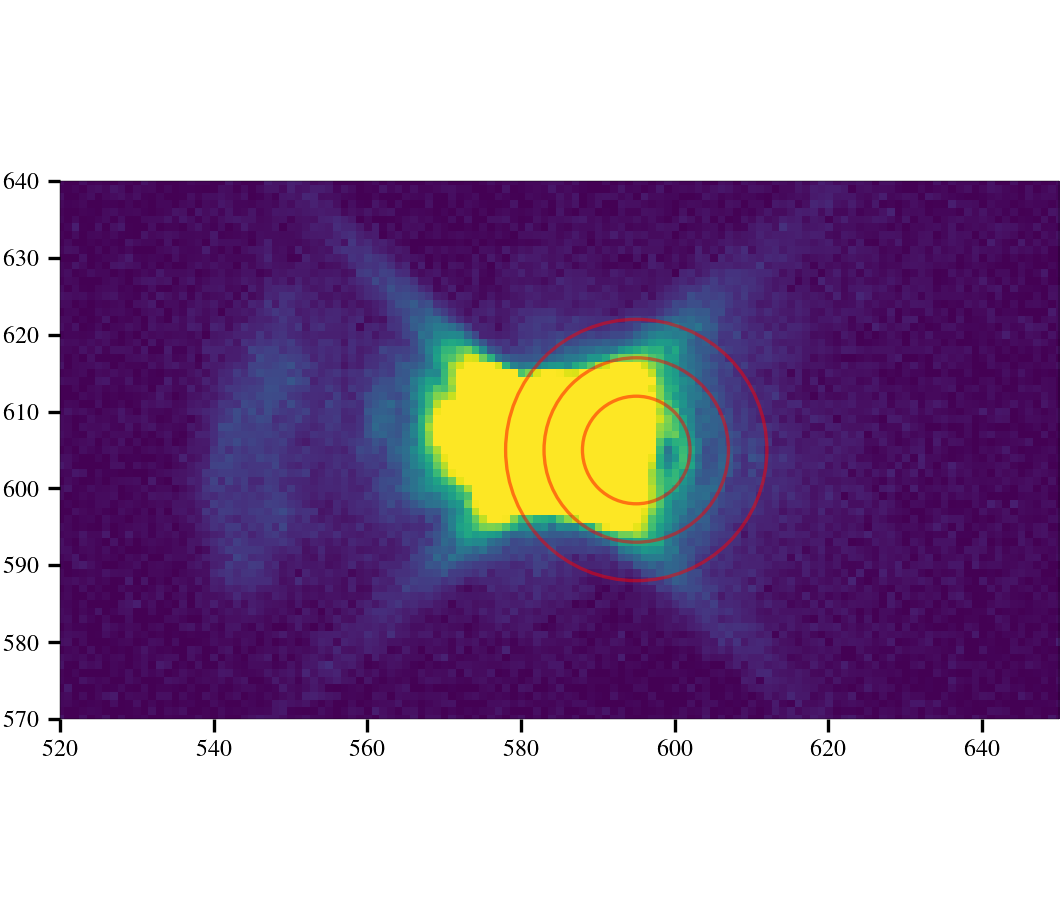
\includegraphics[width=1\linewidth]{fig/diffraction_dust.png}
  \caption{Diffraction rings due to the presence of a dust spot on the r filter. Red circles are over-plotted to ease the visualisation.}
  \label{fig:dust}
\end{figure}


Overall, the model provides a satisfactory description of the
dataset. The most significant discrepancy is a noticeable gray
decrease of the transmission of the $r$ filters for the sample
measurement at \SI{3.7}{\degree} with respect to the average of the
other three.  After investigating this issue, we identified that PSF
tails in the corresponding images displayed a diffraction figure
consistent with a dust particle on the filter surface intercepting the
beam. Based on the approximate area of the beam spot
($\sim\SI{12}{mm^2}$), and the estimated particle size range (between
\SIrange{200}{300}{\micro\metre}), we calculated a potential decrease
in transmission of up to ~$\SI{0.6}{\percent}$. This value aligns well
with the observed decrease. Similar discrepancies were found for some
observations in $u$, $g$ and $y$ bands, although determining particle
sizes from diffraction features was not possible in these cases. We
attribute these discrepancies to dust contamination on the filter
surface as well.

The top panel of Fig.~\ref{fig:metrics} shows the difference between
the transmission integral for measurements and the model at each
position, helping readers better visualize the 'gray'
discrepancies. The standard deviation of model/measurement
discrepancies is ~$\SI{10.2}{mmag}$. Considering this value as an
estimate of dust-induced dispersion, we can deduce that the
corresponding uncertainty for per-filter normalization of the model
(averaging 4 independent samples) is approximately $\SI{5}{mmag}$.

This noise could be decreased by averaging more sample measurements of
the mirror. In our case 4 additionnal positions were sampled as part
of run 3 (see table~\ref{tab:schedule}). However, while run 2
measurements were carefully taken to sample the mirror from the outer
edge to the inner edge along a radius with separations provided by the
mount encoders, the other measurements were positioned semi-randomly
with the idea that the position of the CCD-window ghost in the images
will enable precise determination of the position of the beam in the
mirror. Two issues were overlooked at this stage which complicate the
determination of the geometry from the position of the ghosts: (1) The
wedge of the window and (2) the ghost positions depend of the
conjugation relation between the CBP and the telescope

The bottom panel in Fig.~\ref{fig:metrics} displays the difference
between the measured central wavelength and the model-predicted value
for all 4 radius positions. The model accurately reproduces the
central wavelengths of all filters with a standard deviation of only
$\SI{0.13}{nm}$. This represents an improvement by an order of
magnitude compared to a model that neglects wavelength shift
considerations, highlighting the importance of including this effect
in the StarDICE response model.

\begin{figure}
  \centering
  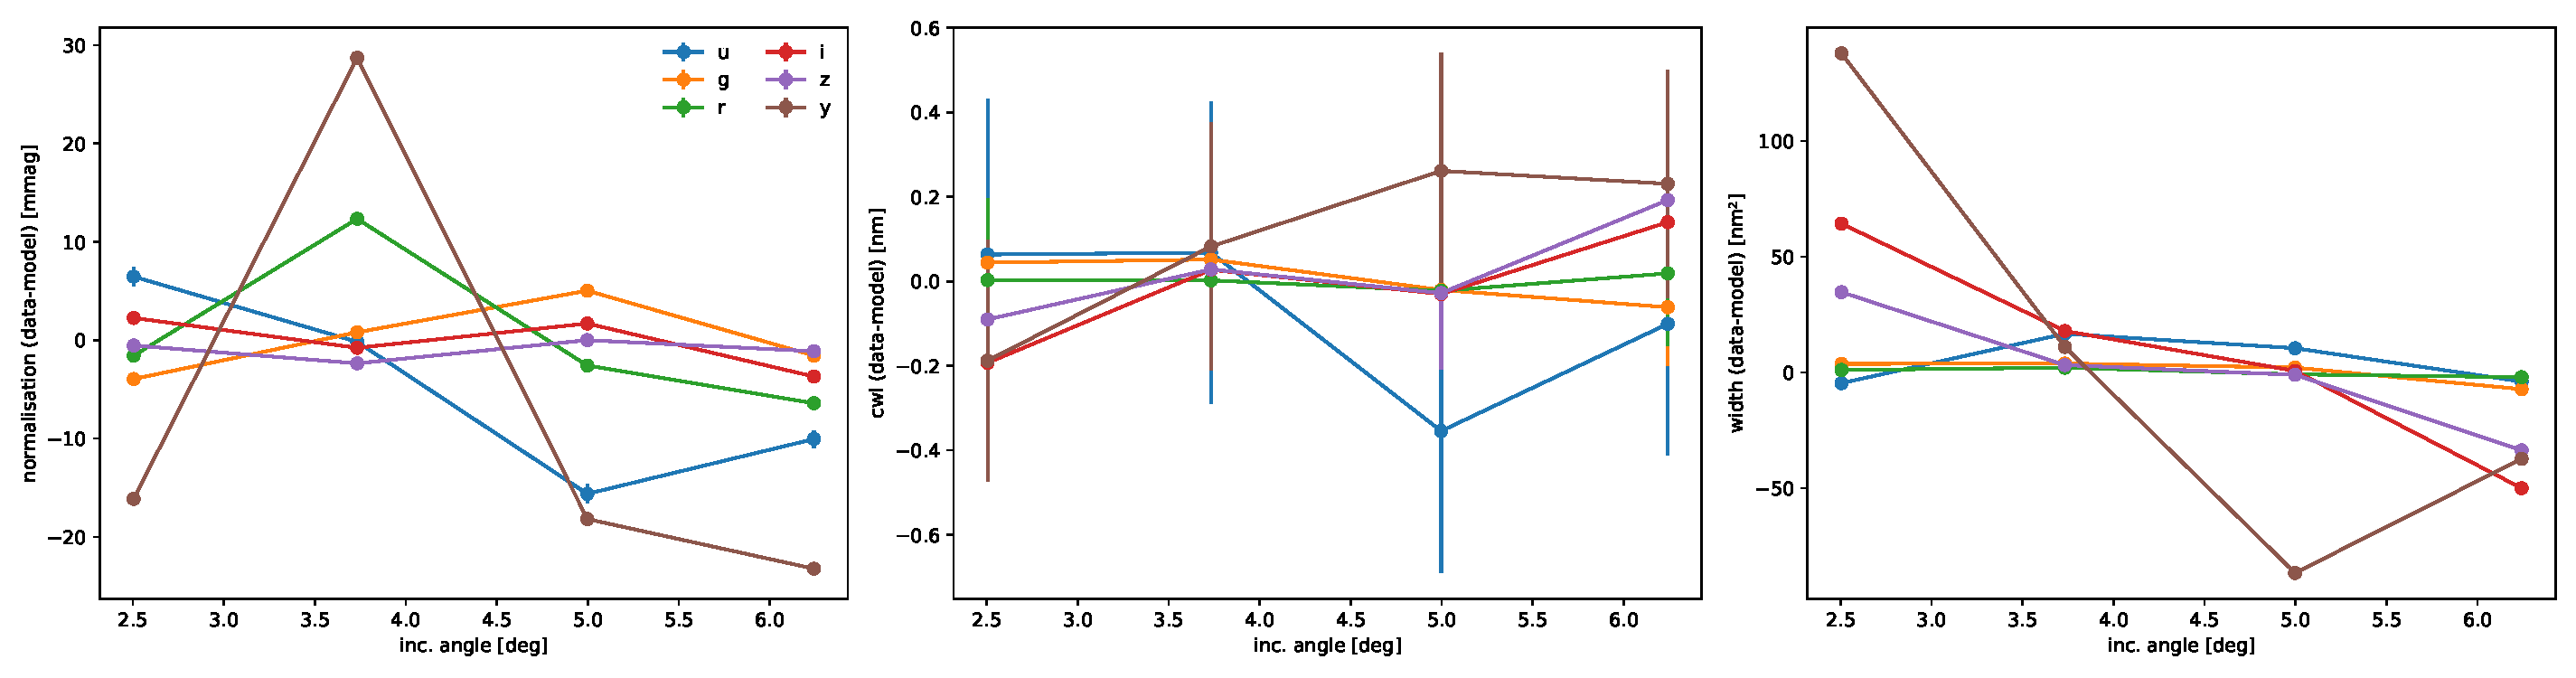
\includegraphics[width=1\linewidth]{fig/metrics.pdf}
  \caption{Discrepancies between model and raw measurements at different mirror locations summarized according to 3 metrics: summarize}
  \label{fig:metrics}
\end{figure}

\subsection{Full pupil synthetic transmission curves}

The full pupil transmission is synthesized by numerically averaging
the above model assuming that the pupil is a perfect annulus with an
inner radius of \SI{55}{mm} and an outer radius of \SI{203}{mm}. A
rectangular quadrature with 100 evenly sampled points in radius has
been used for the averaging. The curves have been normalized using the
CBP response from Sect.\ref{sec:cbp}. An estimate of the
absolute transmission curve is then computed assuming an effective
mirror area of TX. The resulting transmission curves are shown in
Fig.~\ref{fig:fullpupiltrans}.
\begin{figure}
  \centering
  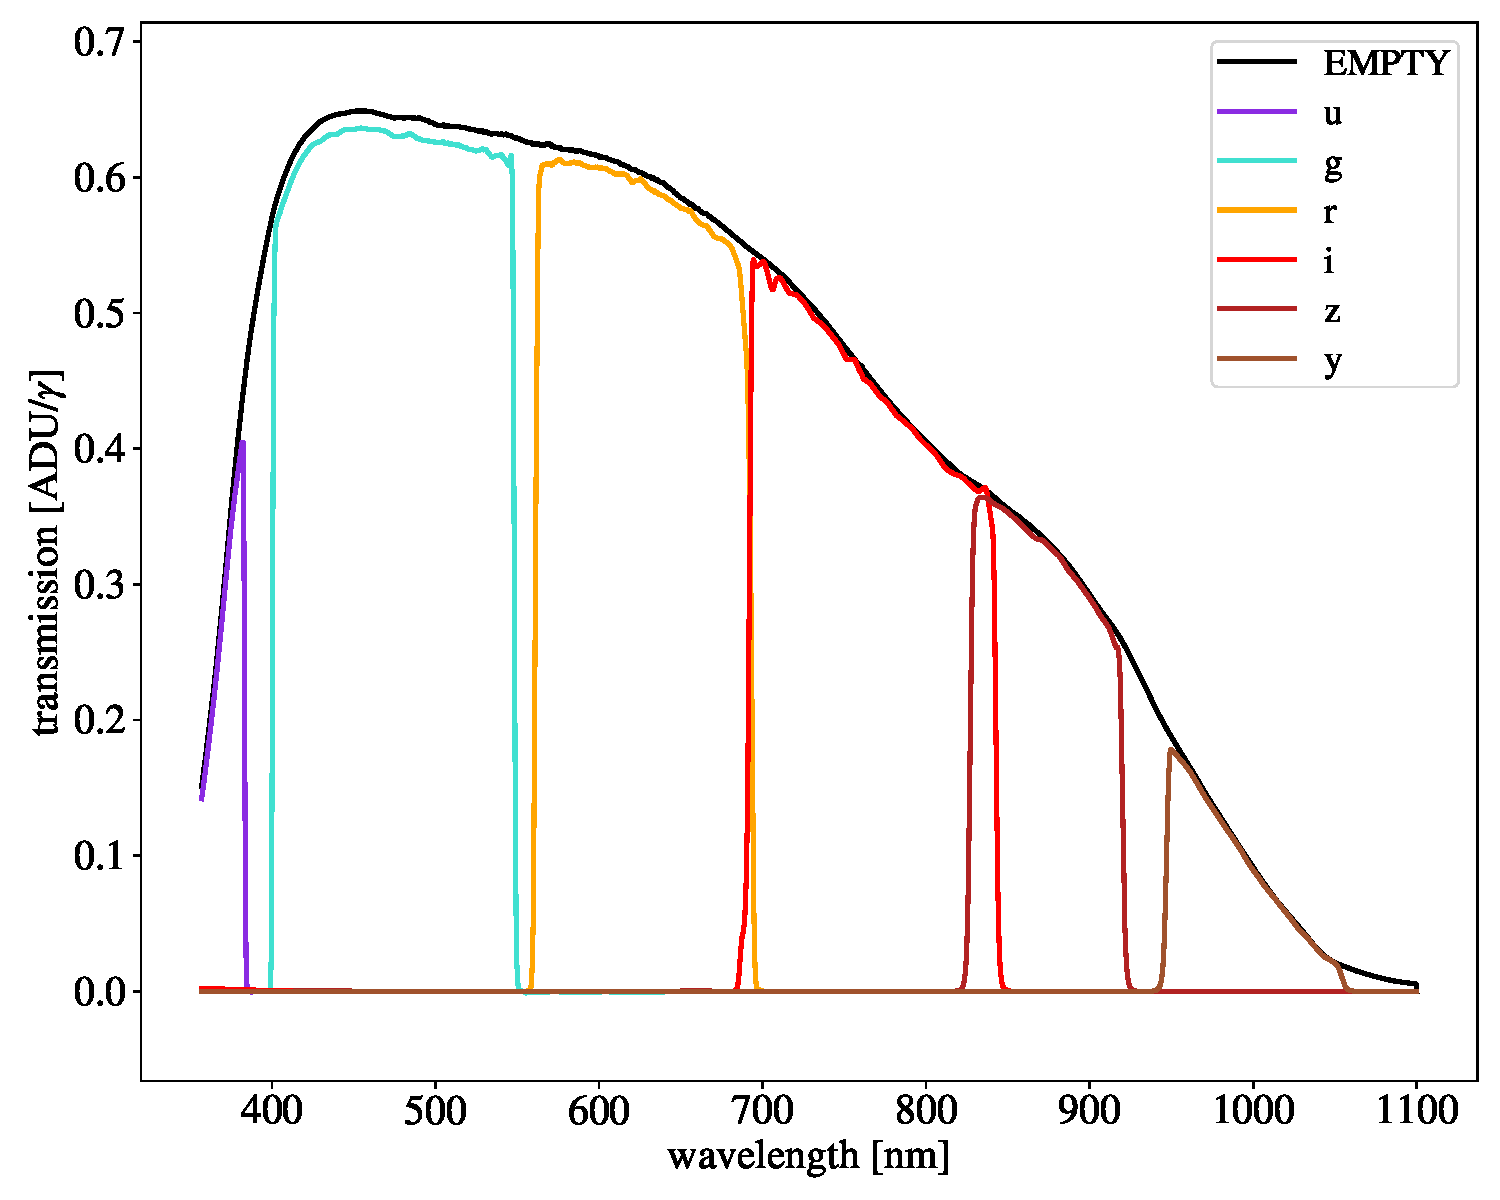
\includegraphics[width=1\linewidth]{fig/fullpupill.pdf}
  \caption{Full-pupil transmission curves for the StarDICE instruments.}
  \label{fig:fullpupiltrans}
\end{figure}


\subsection{Final error budget}

We present the impact of the various uncertainty sources on absolute
stellar fluxes in Table~\ref{tab:budget}.
\begin{table}
  \centering
  \caption{Relative uncertainty on the synthetic magnitudes of
    G191B2B, split by contributions.}
  \label{tab:budget}
\begin{tabular}{lrrrrrr}
  \toprule
  \toprule
  source & u & g & r & i & z & y \\
  $[$mmag$]$\\
  \midrule
  StarDICE & 0.5 & 0.2 & 0.2 & 0.3 & 1.0 & 3.8 \\
  $\eta_{SC}$ & 1.6 & 0.1 & 0.1 & 0.1 & 0.1 & 0.1 \\
  CBP & 2.2 & 0.5 & 1.2 & 0.0 & 0.0 & 0.1 \\
  \midrule
  Stat (total) & 2.7 & 0.5 & 1.2 & 0.3 & 1.0 & 3.8 \\
  \midrule
  Scattered light & 2.7 & 3.1 & 3.8 & 4.3 & 4.8 & 5.3 \\
  Repeatability & 0.8 & 0.4 & 0.5 & 1.1 & 1.1 & 1.1 \\
  Linearity & 0.2 & 0.2 & 0.3 & 0.5 & 0.5 & 0.5 \\
  Contamination & 4.4 & 0.6 & 0.8 & 0.1 & 0.1 & 0.1 \\
  Mirror sampling noise & 5.4 & 5.4 & 5.4 & 5.4 & 5.4 & 5.4 \\
  \midrule
  Syst (total) & 7.5 & 6.3 & 6.7 & 7.0 & 7.4 & 7.7 \\
  \midrule
  Total & 8.0 & 6.3 & 6.8 & 7.1 & 7.4 & 8.6 \\
%  \bottomrule
\end{tabular}
\end{table}

\begin{figure}
  \centering
  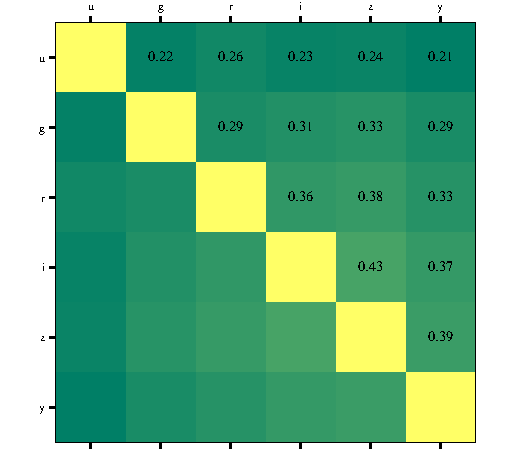
\includegraphics[width=1\linewidth]{fig/bandcorrelation.pdf}
  \caption{Correlation of the uncertainties on the synthetic magnitudes of G191B2B.}
  \label{fig:correlation}
\end{figure}
